\documentclass[leqno]{article}
\usepackage[utf8x]{inputenc}
\usepackage[T1]{fontenc}
\usepackage{amsfonts}
\usepackage{enumerate}
\author{Colin Roberts}
\title{MATH 546, Homework 4}
\usepackage[left=3cm,right=3cm,top=3cm,bottom=3cm]{geometry}
\usepackage{amsmath}
\usepackage[thmmarks, amsmath, thref]{ntheorem}
%\usepackage{kbordermatrix}
\usepackage{mathtools}
\usepackage{color}
\usepackage{hyperref}
\usepackage{tikz-cd}
\usepackage{float}
\usepackage{morefloats}
\usepackage{graphicx}
\usetikzlibrary{quotes,arrows.meta}
\tikzset{
  annotated cuboid/.pic={
    \tikzset{%
      every edge quotes/.append style={midway, auto},
      /cuboid/.cd,
      #1
    }
    \draw [every edge/.append style={pic actions, densely dashed, opacity=.5}, pic actions]
    (0,0,0) coordinate (o) -- ++(-\cubescale*\cubex,0,0) coordinate (a) -- ++(0,-\cubescale*\cubey,0) coordinate (b) edge coordinate [pos=1] (g) ++(0,0,-\cubescale*\cubez)  -- ++(\cubescale*\cubex,0,0) coordinate (c) -- cycle
    (o) -- ++(0,0,-\cubescale*\cubez) coordinate (d) -- ++(0,-\cubescale*\cubey,0) coordinate (e) edge (g) -- (c) -- cycle
    (o) -- (a) -- ++(0,0,-\cubescale*\cubez) coordinate (f) edge (g) -- (d) -- cycle;
    \path [every edge/.append style={pic actions, |-|}]
    (b) +(0,-5pt) coordinate (b1) edge ["\cubex \cubeunits"'] (b1 -| c)
    (b) +(-5pt,0) coordinate (b2) edge ["\cubey \cubeunits"] (b2 |- a)
    (c) +(3.5pt,-3.5pt) coordinate (c2) edge ["\cubez \cubeunits"'] ([xshift=3.5pt,yshift=-3.5pt]e)
    ;
  },
  /cuboid/.search also={/tikz},
  /cuboid/.cd,
  width/.store in=\cubex,
  height/.store in=\cubey,
  depth/.store in=\cubez,
  units/.store in=\cubeunits,
  scale/.store in=\cubescale,
  width=1,
  height=1,
  depth=1,
  units=,
  scale=2,
}

\theoremstyle{nonumberplain}
\theoremheaderfont{\itshape}
\theorembodyfont{\upshape:}
\theoremseparator{.}
\theoremsymbol{\ensuremath{\square}}
\newtheorem{proof}{Proof}
\theoremsymbol{\ensuremath{\square}}
\newtheorem{lemma}{Lemma}
%\theoremsymbol{\ensuremath{\square}}
\newtheorem{solution}{Solution}
%\theoremseparator{. ---}
%\theoremsymbol{\mbox{\texttt{;o)}}}
%\newtheorem{varsol}{Solution (variant)}

\newcommand{\id}{\mathrm{Id}}
\newcommand{\im}{\mathrm{im}}
\newcommand{\R}{\mathbb{R}}
\newcommand{\N}{\mathbb{N}}
\newcommand{\Z}{\mathbb{Z}}
\newcommand{\C}{\mathbb{C}}
\newcommand{\RE}{\textrm{Re}}
\newcommand{\IM}{\textrm{Im}}

\newcommand{\End}{\mathrm{End}}

% Matlab code
\usepackage{listings}
\usepackage{color} %red, green, blue, yellow, cyan, magenta, black, white
\definecolor{mygreen}{RGB}{28,172,0} % color values Red, Green, Blue
\definecolor{mylilas}{RGB}{170,55,241}

\begin{document}
\maketitle
\begin{large}
\begin{center}
Solutions
\end{center}
\end{large}

%%%%%%%%%%%%%%%%%%%%%%%%%%%%%%%%%%%%%%%%%%%%%%%%%%%%%%%%%%%%%%%%%%%%%%%%%%%%%%%%%%%%%%%%%%%%%%%%%%%%%%%%%%%%%%%%%%%%%
%%%%%%%%%%%%%%%%%%%%%%%%%PROBLEM%%%%%%%%%%%%%%%%%%%%%%%%%%%%%%%%%%%%%%%%%%%%%%%%%%%%%%%%%%%%%%%%%%%%%%%%%%%%%%%%%%%%%%%%%%%%%%%%%%%%%%%%%%%%%%%%%%%%%%%%%%%%%%%%%%%%%%%%%%%%%%%%%%%%%%%%%%%%%%%%%%%%%%%%%%%%%%%%%%%%%%%%%%%%%%%%%%%%%%%%%%

\paragraph{Problem 1 (The space $H^{1/2}$, take 1: Via the Fourier transform).}
If one thinks of the space $H^k$ as the space of functions that have
$k$ square integrable (weak) derivatives, then $H^{1/2}$ would be the
space of functions that have half a derivative. This is hard to
understand in terms of what such a half derivative should actually be,
but we can define it as follows: Recall that the Fourier
transformation satisfies the property
\begin{align*}
  {\cal F}\left[ \frac{d^j}{dx^j} f(x) \right](k)
  &=
  \frac{1}{\sqrt{2\pi}}
  \int_{-\infty}^{\infty} \left[ \frac{d^j}{dx^j} f(x) \right] e^{ikx}
  \, \text{d}x
  \\
  &=
  (-1)^j
  \frac{1}{\sqrt{2\pi}}
  \int_{-\infty}^{\infty} f(x) \left[ \frac{d^j}{dx^j} e^{ikx}\right] 
  \, \text{d}x
  \\
  &=
  (-1)^j
  \frac{1}{\sqrt{2\pi}}
  \int_{-\infty}^{\infty} f(x) (ik)^j e^{ikx}
  \, \text{d}x
  \\
  &=
  (-ik)^j
  \frac{1}{\sqrt{2\pi}}
  \int_{-\infty}^{\infty} f(x) e^{ikx}
  \, \text{d}x
  \\
  &=
  (-ik)^j {\cal F}[f](k).
\end{align*}
The key step here was simply the integration by parts from the first
to the second line.

Because the Fourier transform is invertible, we also have
\begin{align*}
  \frac{d^j}{dx^j} f
  = {\cal F}^{-1}\left({\cal F}\left[ \frac{d^j}{dx^j} f \right]\right)
  &=
  {\cal F}^{-1}\left((-ik)^j {\cal F}[f]\right).
\end{align*}
This formula is useful because we can now talk about what it means to
take a half-derivative: we just choose $j=1/2$ in this last formula --
we can then compute $\left(\frac{d}{dx}\right)^{1/2} f$ by just doing
the forward and inverse Fourier transform. Of course, this can also be
done with any other $j$, whether it is an integer or not, and whether
it is positive or not.

So let's come back to the original question: Is the step function
\begin{align*}
  h(x)
  =
  \begin{cases} 
    0 & \text{if $x<0$}, \\
    1 & \text{if $x\ge 0$}
  \end{cases}
\end{align*}
defined on the interval $\Omega=(-1,1)$ in the space
$H^{1/2}(\Omega)$? As usual, we will say that a function $u$ is in
$H^s(0,1)$ if it is in $L^2$ and its $s$th derivative is square
integrable.

To answer this question, you will need
to figure out whether $\left(\frac{d}{dx}\right)^{1/2} h$ is square
integrable. For this, you have to (i) find the Fourier transform of
$h$ (which here is really just a Fourier series, because your domain
is finite), and (ii) use the
\href{https://en.wikipedia.org/wiki/Plancherel_theorem}{Plancherel
  identity} that says that the $L^2$ norm of a function and the $L^2$
norm of its (inverse) Fourier transform are equal (potentially up to a
constant, depending on how exactly one defines the Fourier
transform). The latter is useful because you won't have to do the
awkward inverse Fourier transform.

While you're there, answer the following question:
\begin{itemize}
  \item If your answer is that $h\in H^{1/2}$, then is $h$ also in the
    spaces $H^{1/2+\varepsilon}$ for any $\varepsilon>0$?
  \item If your answer is that $h\not\in H^{1/2}$, then is $h$ at
    least in the spaces $H^{1/2-\varepsilon}$ for any $\varepsilon>0$?
\end{itemize}

\begin{solution}
Note that we can take the Fourier representation of $h(x)$ by
\[
h(x) = \frac{1}{2} + \frac{2}{\pi} \sum_{n=0}^\infty \frac{1}{2n+1} \sin((2n+1)\pi x).
\]
Then, if we take
\[
\mathcal{F}(h)(k) = \frac{2}{\pi (2k+1)}.
\]
So then we have that
\[
\mathcal{F}\left(\frac{d^{1/2}}{dx^{1/2}}h\right)(k) = (-ik)^{1/2} \frac{2}{\pi(2k+1)} ~~\textrm{for $k=0,1,\dots$}.
\]
Then using Plancherel (that $\mathcal{F}$ is unitary), we check that $\mathcal{F}\left(\frac{d^{1/2}}{dx^{1/2}}h\right)(k)$ is square integrable by
\begin{align*}
\int_{-\infty}^\infty \mathcal{F}\left(\frac{d^{1/2}}{dx^{1/2}}h\right)(k) dk = \sum_{k=0}^\infty \left|(-ik)^{1/2} \frac{2}{\pi(2k+1)}\right|^2 &= \sum_{k=0}^\infty \frac{4k}{\pi^2(2k+1)^2} = \infty.
\end{align*}
However, for $j=1/2-\epsilon$ we have
\[
\sum_{k=0}^\infty \frac{4k^{-2\epsilon}}{\pi^2(2k+1)^2}<\infty
\]
by a comparison test to a convergent $p$-series.  The idea here is that the terms we sum over decay like $\frac{1}{j^\epsilon}$ and so the series converges.

\end{solution}
\pagebreak



\paragraph{Problem 2 (The space $H^{1/2}$, take 2: Slobodeckij's definition).}
Let's take a different definition of $H^{s}$ where $s$ may not be an
integer: We say that a function $u\in L^2$ is in the space $H^{s}$ if
its $H^{s}$-norm is finite, where this norm is defined as follows:
\begin{align*}
  \|u\|_{H^s(\Omega)} = \int_\Omega \int_\Omega
  \frac{|u(x)-u(y)|^2}{|x-y|^{2s+d}} \text{d}y \, \text{d}x.
\end{align*}
Here, $d$ is the dimension of the domain $\Omega$. Again, this
definition (originally given by Slobodeckij) is valid for arbitrary
$0<s<1$. (If you wanted to define the space $H^{3/2}$ in this way,
you'd check that $u\in H^1$ and that $\nabla u\in H^{1/2}$.)

Answer the same questions as for Problem 1:
\begin{itemize}
  \item Is $h\in H^{1/2}$ using this definition of the space?
  \item If your answer is that $h\in H^{1/2}$, then is $h$ also in the
    spaces $H^{1/2+\varepsilon}$ for any $\varepsilon>0$?
  \item If your answer is that $h\not\in H^{1/2}$, then is $h$ at
    least in the spaces $H^{1/2-\varepsilon}$ for any $\varepsilon>0$?
\end{itemize}

\begin{solution}
We take
\begin{align*}
    \|h\|_{H^{1/2}} &= \int_{-1}^1 \int_{-1}^1 \frac{|h(x)-h(y)|^2}{|x-y|^2}dydx\\
    &= \int_{-1}^1 \left[ \int_{-1}^0 \frac{|h(x)|^2}{|x-y|^2}dy + \int_0^1 \frac{|h(x)-1|^2}{|x-y|^2}dy\right]dx.
\end{align*}
Note that we have $|x-y|^2=x^2-2xy+y^2$ and thus we have
\begin{align*}
\|h\|_{H^{1/2}} &= \int_{-1}^1 \frac{|h(x)|^2}{x^2+x}dx+\int_{-1}^1 \frac{|h(x)-1|^2}{x^2-x}dx\\
&= \int_0^1 \frac{1}{x^2+x}dx + \int_{-1}^0 \frac{1}{x^2-x}dx.
\end{align*}
Note that both of these integrals diverge (with positive value), thus we have that $h\notin H^{1/2}$ by this definition.

Now, if we consider $H^{1/2-\epsilon}$, then we check
\begin{align*}
\|h\|_{H^{1/2-\epsilon}} &= \int_{-1}^1 \int_{-1}^1 \frac{|h(x)-h(y)|^2}{|x-y|^{2-2\epsilon}}dydx\\
&= \int_{-1}^1 \left( \int_{-1}^0 \frac{|h(x)|^2}{|x-y|^{2-2\epsilon}}dy \int_0^1 \frac{|h(x)-1|^2}{|x-y|^{2-2\epsilon}}dy \right)dx\\
&= \int_0^1 \int_{-1}^0 \frac{1}{|x-y|^{2-2\epsilon}}dydx + \int_{-1}^0 \int_0^1 \frac{1}{|x-y|^{2-2\epsilon}}dydx\\
&= \int_0^1 \int_{-1}^0 \frac{1}{(x-y)^{2-2\epsilon}} dydx + \int_{-1}^0 \int_0^1 \frac{1}{(x-y)^{2-2\epsilon}} dydx &&\textrm{since $x-y$ will be positive},\\
&= \frac{2-4^\epsilon}{\epsilon-2\epsilon^2}.
\end{align*}
Then note that we have
\[
\frac{2-4^\epsilon}{\epsilon-2\epsilon^2}<\infty 
\]
for any $\epsilon>0$.
\end{solution}
\pagebreak

\paragraph{Problem 3 (The space $H^{1/2}$, take 3).}
The last way we'll consider here in which one could define the space
$H^{1/2}(\Omega)$ on a one-dimensional domain $\Omega$ is a bit
backward because it doesn't quite give a statement one can easily
check. It assumes that the one-dimensional domain $\Omega$ is (a
subset of) the boundary of a two-dimensional domain $\Sigma\subset\R^2$, i.e.,
$\Omega\subset\partial\Sigma$. Since we're considering
$\Omega=(-1,1)$, we can for example choose $\Sigma=(-1,1)^2$.

Then take a close look at the following statement: We define
$H^{1/2}(\Omega)$ as
\begin{align*}
  H^{1/2}(\Omega) = \left\{
    \varphi\in L^2(\Omega) : \text{there exists $u\in H^1(\Sigma)$ so
      that $T_\Omega u = \varphi$}
  \right\}.
\end{align*}
Here, $T_\Omega$ is the trace operator that takes the boundary values
of $u$ on the part of the boundary of $\Sigma$ that is $\Omega$. In
other words, $H^{1/2}(\Omega)$ is the set of all possible boundary
values that functions $u\in H^1(\Sigma)$ can have. You'll note that
unlike the two other definitions, this one really is specific to an
index of 1/2 and can't easily be generalized to other fractional
values.

As before, check whether $h\in H^{1/2}(\Omega)$ using this definition.



\begin{solution}
Consider $\Sigma=\{(x,y)\in \R^2 ~\vert~ x^2+y^2\leq 1, ~ y\geq 0\}\setminus \{(0,0)\}$ and note that $\Omega\subset \partial \Sigma$.  Then we can view this with polar coordinates and consider the function
\[
u(r,\phi) = \cos\left(\frac{\phi}{2}\right).
\]
We then have that 
\[
Tu|_{(-1,0)} = \lim_{\phi \to \pi} u(r,\phi) = 0
\]
and 
\[
Tu|_{(0,1)} = \lim_{\phi \to 0} u(r,\phi) = 1.
\]
So we have 
\[
Tu = h ~\textrm{almost everywhere.}
\]
So it follows that $h\in H^{1/2}$.

However, this relies on the fact that the chosen $u\in H^1(\Sigma)$ which is not clear.  Take
\[
\nabla u = \begin{bmatrix} 0 \\ \frac{1}{2r} \sin\left(\frac{\phi}{2}\right) \end{bmatrix}.
\]
Then
\begin{align*}
    \int_{\Sigma} \|\nabla u \|^2 rdrd\phi &= \int_\Sigma \frac{1}{4r^2}\sin^2\left(\frac{\phi}{2}\right)rdrd\phi\\
    &\propto \int_\Sigma \frac{1}{r}dr,
\end{align*}
which diverges.
\end{solution}
\pagebreak


\paragraph{Problem 4 (The spaces $H^{k}$ and their Fourier basis).}
We briefly talked about this in class: Just like $\R^n$, one can give
the spaces $H^k$ a \textit{basis}. There are of course many bases one
could choose, but the simplest one (and in many situations the most
\textit{convenient} one) is the Fourier basis.

For this purpose, let's stay in 1d and for convenience choose
$\Omega=(0,2\pi)$. Then every function in $H^k_0(\Omega)$ can be
written as
\begin{align*}
  u(x) = \sum_{j=1}^\infty a_j \sin(jx) = a_1 \sin(x) + a_2 \sin(2x) + \ldots
\end{align*}
Prove the following statements:
\begin{enumerate}
\item If the coefficients $a_j$ of a function $u(x)$ satisfy the condition 
$|a_j| = o\left(\frac{1}{\sqrt{j}}\right)$ -- that is, if 
$\lim_{j\rightarrow\infty}\frac{|a_j|}{1/\sqrt{j}}=0$ -- then $u\in L^2(\Omega)$.

\item If the coefficients $a_j$ of a function $u(x)$ satisfy the condition 
$|a_j| = o\left(\frac{1}{j^{3/2}}\right)$ then $u\in H^1(\Omega)$.

\item If the coefficients $a_j$ of a function $u(x)$ satisfy the condition 
$|a_j| = o\left(\frac{1}{j^{k+1/2}}\right)$ for some $k\ge 0$, then $u\in H^k(\Omega)$.
\end{enumerate}
This last condition also allows us to define membership in spaces
$H^k$ where $k$ is not an integer. This is of course what we did in
Problem 1.

\begin{solution}~
\begin{enumerate}
    \item Take
    \begin{align*}
        \|u\|_{L^2}^2=\int_\Omega |u(x)|^2dx &= \int_0^{2\pi} \left| \sum_{j=1}^\infty a_j \sin(jx)\right|^2 dx\\
        &\leq \int_0^{2\pi} \left| \sum_{j=1}^\infty a_j\right|^2dx &&\textrm{since $-1\leq \sin(jx)\leq 1~\forall x$},\\
        &\leq \int_0^{2\pi} \sum_{j=1}^\infty |a_j|^2 dx\\
        &=\sum_{j=1}^\infty |a_j|^2 \int_0^{2\pi} dx\\
        &=2\pi \sum_{j=1}^\infty |a_j|^2.
    \end{align*}
    Then, since $|a_j|=o\left(\frac{1}{j^{1/2+\epsilon}}\right)$ we have that $|a_j|^2=o\left(\frac{1}{j^{1+\epsilon}}\right)$.  Thus we have a convergent $p$-series
    \[
    \|u\|_{L^2}^2 \leq 2\pi \sum_{j=1}^\infty |a_j|^2 < \infty.
    \]
    \item Take
    \[
    \|u\|_{H^1}^2 = \|u\|_{L^2}^2+\|\nabla u\|_{L^2}^2.
    \]
    Note that $|a_j|=o\left(\frac{1}{j^{3/2+\epsilon}}\right)$ which by the previous work shows that
    \[
    \|u\|_{L^2}^2<\infty.
    \]
    Hence, it suffices to show that
    \[
    \|\nabla u\|_{L^2}^2<\infty.
    \]
    Now, since $u(x)$ is periodic and continuous since $u\in H_0^k(\Omega)$ we can compute
    \[
    \nabla u(x) = \sum_{j=1}^\infty ja_j\cos(jx).
    \]
    So we have
    \begin{align*}
        \|\nabla u\|_{L^2}^2 &= \int_0^{2\pi} \left| \sum_{j=1}^\infty ja_j \cos(jx)\right|^2dx\\
        &\leq \int_0^{2\pi} \left|\sum_{j=1}^\infty ja_j\right|^2dx\\
        &\leq 2\pi \sum_{j=1}^\infty j^2|a_j|^2.
    \end{align*}
    Then, since $|a_j|=o\left(\frac{1}{j^{3/2+\epsilon}}\right)$ we have that
    \[
    j^2|a_j|^2 = o\left( \frac{j^2}{j^{3+\epsilon}}\right)=o\left(\frac{1}{j^{1+\epsilon}}\right)
    \]
    and hence our series above is a convergent $p$-series.  Thus it follows that $u\in H^1(\Omega)$.
    \item By an inductive argument, one can see that the highest order derivative requires the most restriction on the decay rate of the coefficients.  Hence, if we wish to show $u\in H^k(\Omega)$ it suffices to show
    \[
    \|\nabla^k u\|_{L^2}^2<\infty.
    \]
    Assuming we can do term by term derivatives, we note that we have
    \[
    \nabla^k u(x) \leq \sum_{j=1}^\infty j^k |a_j|
    \]
    as there is either a $\sin(jx)$ or $\cos(jx)$ term but each is bounded by $1$ in absolute value.  So we have
    \begin{align*}
        \|\nabla^k u\|_{L^2}^2 &\leq 2\pi \sum_{j=1}^\infty j^{2k} |a_j|^2,
    \end{align*}
    and since we have $|a_j|=o\left(\frac{1}{j^{k+1/2+\epsilon}}\right)$ we have
    \[
    j^{2k}|a_j|^2 = o\left(\frac{j^{2k}}{j^{2k+1+\epsilon}}\right)=o\left(\frac{1}{j^{1+\epsilon}}\right).
    \]
    Again, we have a convergent $p$-series so $u\in H^k(\Omega)$.
\end{enumerate}
\end{solution}
\pagebreak

\paragraph{Bonus problem (The space $H^{-1}$ and its Fourier basis).}
The space of functions $H^{-1}(\Omega)$ is the set of all functions
$u(x)$ so that
\begin{align*}
  \int_\Omega u(x) v(x) \, \text{d}x
\end{align*}
is finite for all possible $v\in H^1$. Take again $\Omega=(0,2\pi)$
and show the following generalization of the results of the previous
problem to the case $k=-1$. In other words, show the following
statement:
\begin{enumerate}
\item If the coefficients $a_j$ of a function $u(x)$ satisfy the condition 
$|a_j| = o\left(\frac{1}{j^{-1+1/2}}\right)$, then $u\in H^{-1}(\Omega)$.
\end{enumerate}
To get an understanding of how such functions look like, generate
sequences of coefficients $a_j$ (for example, chosen randomly in some
way) that satisfy the conditions for $H^1,L^2,H^{-1}$ and plot these
functions. Do they look qualitatively different?

\begin{solution}
If we take functions of the form
\[
u(x) = \sum_{j=1}^\infty a_j \sin(jx)
\]
and
\[
v(x) = \sum_{k=1}^\infty b_k \sin(kx),
\]
then we can consider
\[
\int_{-1}^1 u(x)v(x)dx.
\]
We then have
\begin{align*}
    \int_{-1}^1 uv dx &= \sum_{k=1}^\infty \sum_{j=1}^\infty \int_{-1}^1 a_j b_k \sin(jx)\sin(kx)dx\\
    &= \sum_{k=1}^\infty \sum_{j=1}^\infty \int_{-1}^1a_jb_k \delta_jk dx\\
    &= \sum_{k=1}^\infty \int_{-1}^1 a_kb_k dx\\
    &= 2\sum_{k=1}^\infty a_kb_k<\infty
\end{align*}
since we have that $|a_j|=o\left(\frac{1}{j^{-1+1/2}}\right)$ and $|b_j|=o\left(\frac{1}{j^{3/2+\epsilon}}\right)$ so $|a_jb_j|=o\left(\frac{1}{j^{1+\epsilon}}\right)$.

Let
\[
f(x) = \sum_{j=1}^\infty j^{-7/4} \sin(jx)
\]
so that $f\in H^1(\Omega)$.  The plot is:
\begin{figure}[H]
    \centering
    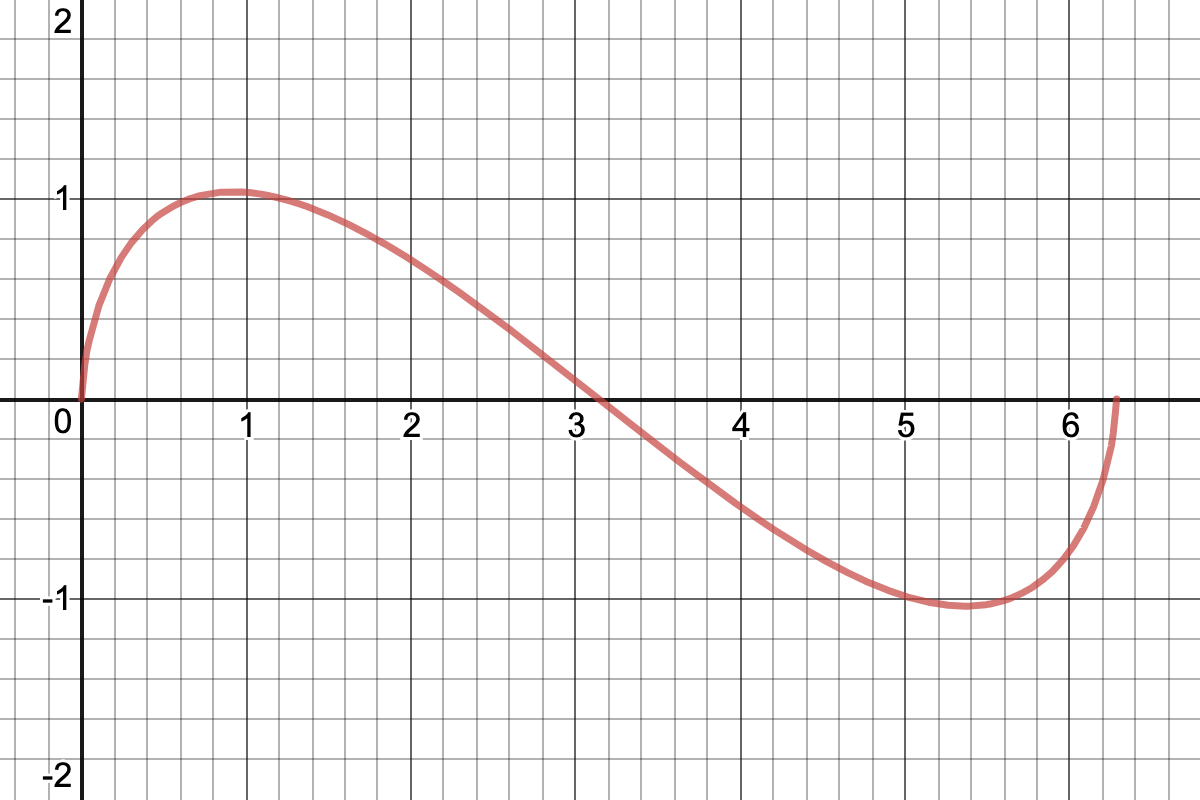
\includegraphics[width=.7\textwidth]{h^1.png}
    \caption{A ``random" $H^1_0(\Omega)$ function.}
\end{figure}

Then let
\[
g(x) = \sum_{j=1}^\infty j^{-3/4} \sin(jx)
\]
so that $g\in L^2(\Omega)$.  The plot is
\begin{figure}[H]
    \centering
    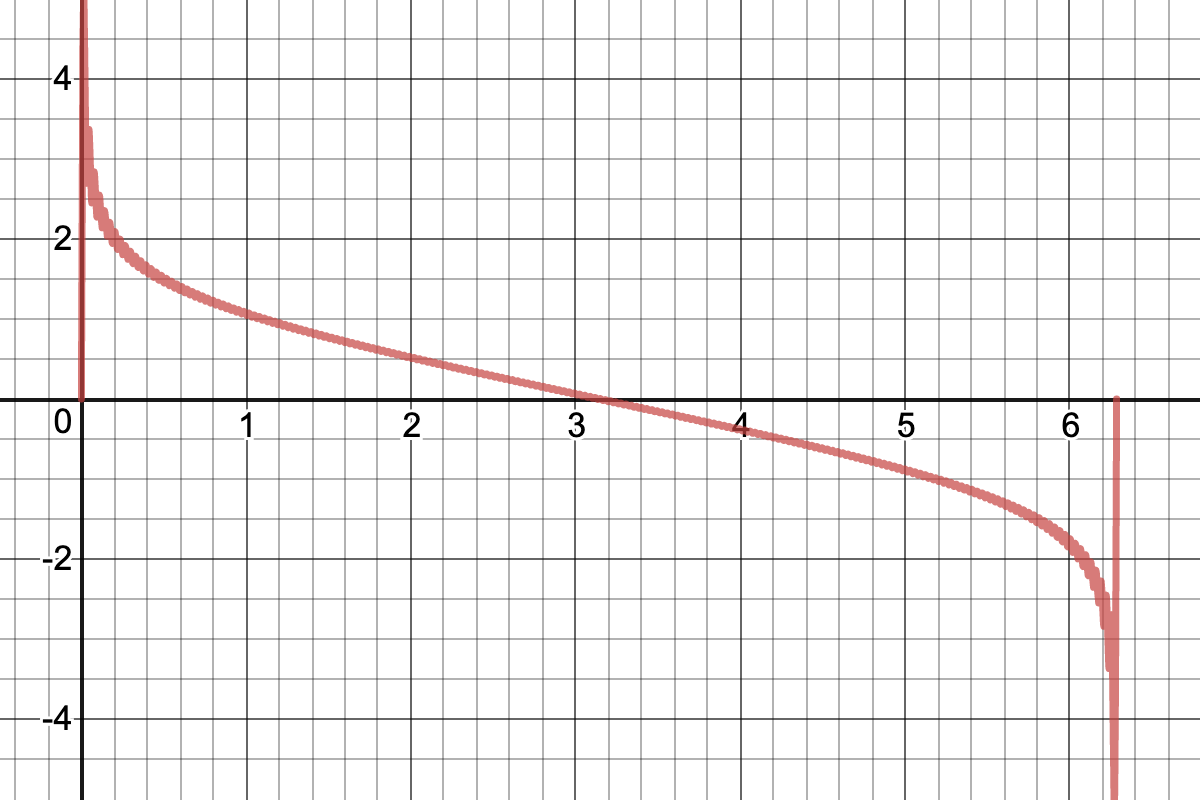
\includegraphics[width=.7\textwidth]{L^2.png}
    \caption{A ``random" $L^2_0(\Omega)$ function.}
\end{figure}

Finally, let
\[
h(x) = \sum_{j=1}^\infty j^{1/4} \sin(jx)
\]
so that $h\in H^1(\Omega)$.  The plot is
\begin{figure}[H]
    \centering
    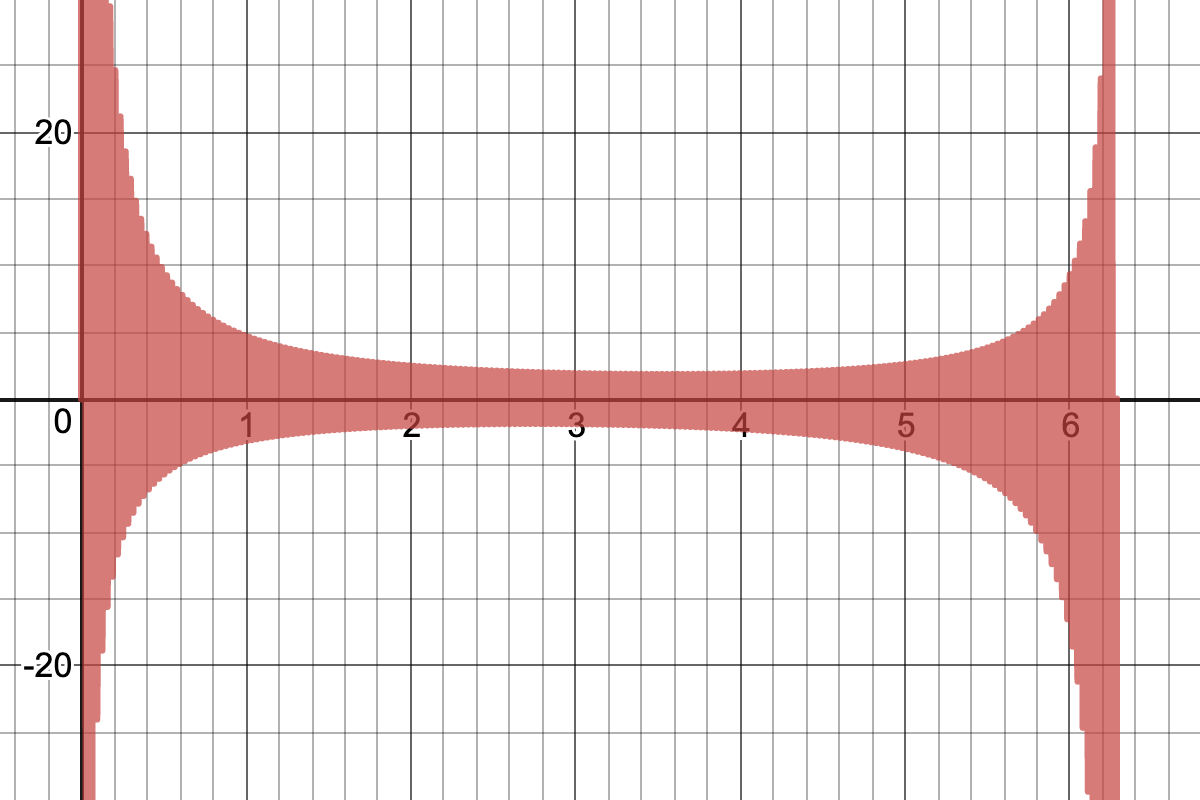
\includegraphics[width=.7\textwidth]{h^-1.png}
    \caption{A ``random" $H^{-1}_0(\Omega)$ function.}
\end{figure}
\end{solution}


\end{document}



